\documentclass[a4paper, openany]{memoir}

\usepackage[utf8]{inputenc}
\usepackage[T1]{fontenc} 
\usepackage[english]{babel}

\usepackage{fancyhdr}
\usepackage{float}

\usepackage{amsmath}
\usepackage{amsthm}
\usepackage{amssymb}
\usepackage{enumitem}
\usepackage{multicol}
\usepackage[bookmarksopen=true,bookmarksopenlevel=2]{hyperref}
\usepackage{tikz}
\usepackage{listings}
\usepackage{xcolor}
\usepackage{indentfirst}
% \usepackage{graphicx}

\pagestyle{fancy}
\fancyhf{}
\fancyhead[LE]{\leftmark}
\fancyhead[RO]{\rightmark}
\fancyhead[RE, LO]{Algorithmics I}
\fancyfoot[LE, RO]{\thepage}
\fancyfoot[RE, LO]{Pete Gautam}

\usetikzlibrary{positioning, automata, arrows}

\definecolor{codegreen}{rgb}{0,0.6,0}
\definecolor{codegray}{rgb}{0.5,0.5,0.5}
\definecolor{codepurple}{rgb}{0.58,0,0.82}
\definecolor{backcolour}{rgb}{0.95,0.95,0.92}

\lstdefinestyle{thestyle}{
    backgroundcolor=\color{backcolour},
    basicstyle=\ttfamily\footnotesize,
    keywordstyle=\color{red!80}\bfseries,
    ndkeywordstyle=\color{blue!80}\bfseries,
    identifierstyle=\color{black},
    commentstyle=\color{codegreen},
    stringstyle=\color{codepurple},
    breakatwhitespace=false,
    breaklines=true,
    captionpos=b,
    keepspaces=true,
    numberstyle=\tiny\color{codegray},
    numbers=left,
    numbersep=2pt,
    showspaces=false,
    showstringspaces=false,
    showtabs=false,          
    tabsize=2
}

\lstdefinelanguage{pseudocode}{ 
    keywords={new, return, this, null, if, in, while, else, for, get, set, class, and, or, not, range},
    ndkeywords={int, char, bool, List, String, Node, Queue, Set, Trie, void, true, false},
    sensitive=true,
    comment=[l]{//},
    morecomment=[s]{/*}{*/},
    morestring=[b]',
    morestring=[b]"
}

\lstset{style=thestyle}

\usetikzlibrary{shapes, positioning}

\chapterstyle{thatcher}

\begin{document}

\chapter{Sorting and Tries}
\setcounter{section}{-1}

\section{Algorithm Analysis}
The time complexity of an algorithm can be thought of as a function of the input size. For example, if we are given an input of size $n$, the time complexity denotes how long it takes for the algorithm to run. It is either the worst case or the average case of the algorithm. 

The worst case analysis is the one specified most commonly. It gives a guarantee of the algorithm's performance. A key factor is the asymptotic behaviour- this indicates what will happen as the input size grows. It is generally expressed using the `Big Oh' notation. In some cases, space complexity can also be significant.

\subsection{Big-Oh notation}
In `Big-Oh' notation, we say that $f(n) = O(g(n))$ if $f$ and $g$ grow at approximately the same rate. Here, the domain of $f$ and $g$ is the natural numbers. Formally, we say that $f(n) = O(g(n))$ if there exists a real constant $c$ and an integer constant $N$ such that $|f(n)| \leq |c \cdot g(n)|$ for all $n \geq N$. Usually, we use this notation to better understand the function $f$; $f$ is typically a complicated function while $g$ is a well-understood function.

When using the `Big-Oh' notation, we use the tightest $g$ that we can. For example, selection sort has worst-case complexity $O(n^2)$. This also means that selection sort is $O(n^3)$, $O(n^4)$, $O(n^2 \log n)$, etc. but we do not say that any of these are the worst-case complexity. However, we cannot state that selection sort is $O(n \log n)$.

\subsection{The logarithmic function}
We say that $x = \log_a n$ if $n = a^x$. The following are few standard properties of the function:
\begin{itemize}
    \item $\log_a m \cdot n = \log_a m + \log_a n$;
    \item $\log_a m/n = \log_a m - \log_a n$;
    \item $\log_a n^c = c \log_a n$.
\end{itemize}
The logarithmic function grows very slowly. For example, $\log_2 1 000 000 \approx 20$. For this reason, $O(n^c \log_2 n)$ is only a little worse than $O(n^c)$.

Using the standard properties of the logarithmic function, we can show that logarithms to different bases related by a constant factor. So, let $x = \log_a n$. In that case, $n = a^x$. Now, if we take $\log_b$ of both sides, we get
\[\log_b n = \log_b a^x = x \log_b a = (\log_a n) \cdot (\log_b a).\]
Since $b$ and $a$ are constants, $\log_b a$ is also a constant. Therefore, $\log_b n$ and $\log_a n$ are related by a constant factor. In terms of `Big-Oh' notation, this implies that $O(\log_a n) = O(\log_b n)$. For this reason, we specify both of these as just $O(\log n)$.

\subsection{Polynomial-time algorithms}
A polynomial-time algorithm runs in $O(n^c)$. The execution time of algorithms with various complexity functions is shown below:
\begin{table}[H]
    \centering
    \begin{tabular}{|c|c|c|c|c|}
        \hline
         & 1 000 & 10 000 & 100 000 & 1 000 000 \\
        \hline
        $n$ & $10^{-6}$ secs & $10^{-5}$ secs & $10^{-4}$ secs & $10^{-3}$ secs \\
        \hline
        $n \log_2 n$ & $10^{-5}$ secs & $1.3 \times 10^{-4}$ secs & $1.6 \times 10^{-3}$ secs & $0.02$ secs \\
        \hline
        $n^2$ & $0.001$ secs & $0.1$ secs & $10$ secs & $16$ mins \\
        \hline
        $n^3$ & $1$ sec & $16$ mins & $11$ days & $32$ years \\
        \hline
    \end{tabular}
    \caption{The execution time of polynomial-time algorithms with various complexity functions provided that we can complete $10^9$ operations per second.}
\end{table}
Clearly, the higher the power, the longer it takes for the algorithm to be solved. Nonetheless, the table above denotes the worst-case behaviour- it is possible for the average case behaviour might be much faster.

\subsection{Exponential-time algorithms}
An exponential-time algorithm runs in $O(c^n)$. The execution time of algorithms with various complexity functions is shown below:
\begin{table}[H]
    \centering
    \begin{tabular}{|c|c|c|c|c|}
        \hline
         & $10$ & $20$ & $30$ & $40$ \\
        \hline
        $2^n$ & $10^{-6}$ secs & $0.001$ secs & $1.1$ secs & $18$ mins \\
        \hline
        $n!$ & $0.004$ secs & $77$ years & $\star$ & $\star$ \\
        \hline
    \end{tabular}
    \caption{The execution time of exponential-time algorithms with various complexity functions provided that we can complete $10^9$ operations per second.}
\end{table}
A star ($\star$) indicates that it takes longer than the age of the Earth for the algorithm to terminate. Looking at the two tables, we can say that polynomial-time algorithms are potentially useful in practice, while exponential-time algorithms are potential useless in practice.
\newpage

\section{Abstract Data Types}
\subsection{Stack}
A stack is an abstract data type that holds a collection of objects. The objects are accessed using a last-in-first-out (LIFO) policy. The basic operations defined on a stack are:
\begin{itemize}
    \item \texttt{create}, which creates an empty stack;
    \item \texttt{isEmpty}, which checks if the stack is empty;
    \item \texttt{push}, which inserts a new item on the top of the stack; and
    \item \texttt{pop}, which removes the item from the top of the stack.
\end{itemize}
We can represent a stack as an array. Here, the bottom of the stack is `anchored' to one end of the array. All the operations are $O(1)$ in that case. We can also represent a stack as a linked list. Again, all the operations are $O(1)$.

\subsection{Queue}
A queue is an abstract data type that too holds a collection of objects. The objects are accessed using a first-in-first-out (FIFO) policy. The basic operations defined on a queue are:
\begin{itemize}
    \item \texttt{create}, which creates an empty queue;
    \item \texttt{isEmpty}, which checks if the queue is empty;
    \item \texttt{insert}, which inserts a new item at the back of the queue; and
    \item \texttt{delete}, which removes the item at the front of the queue.
\end{itemize}
We can represent a queue as an array. We need to wrap the queue around the array so that all the operations are $O(1)$. We can also use a linked list to represent a queue. Again, all the operations are $O(1)$.

\subsection{Priority Queue}
A priority queue is an abstract data type that is very similar to a queue. Instead of holding the elements in the given order, each element has a priority. When removing an element, we remove the one with the highest priority first. We can achieve this by keeping the queue sorted at all times, for example.

The basic operations defined on a priority queue are the same as a queue: \texttt{create}, \texttt{isEmpty}, \texttt{insert} and \texttt{delete}.

If we represent a priority queue as an unordered list, then the operation \texttt{insert} is $O(1)$ while the operation \texttt{delete} is $O(n)$. On the other hand, if we represent it as an ordered list, then the operation \texttt{delete} is $O(1)$ while the operation \texttt{insert} is $O(n)$. If we store it as a heap, then both \texttt{insert} and \texttt{delete} are both $O(\log n)$. In all cases, the other operations \texttt{create} and \texttt{isEmpty} are $O(1)$.
\newpage

\section{Sorting algorithms}
We have seen before that naive sorting algorithms such as selection sort, insertion sort and bubble sort are $O(n^2)$ in worst (or average) case. There are also clever sorting algorithms such as heap sort, merge sort and quick sort that are $O(n \log n)$ in worst (or average) case. In practice, the fastest sorting algorithm is quicksort, even though its worse case is $O(n^2)$. This is because, in practice, the worst case is not encountered often.

The best runtime of these algorithms is $O(n \log n)$. In fact, it is not possible for us to use a comparison-based sorting algorithm with runtime better than $O(n \log n)$.

\subsection{Comparison-based sorting}
The algorithms we have above involve comparing elements to establish the order of the sorted list. For this reason, they are called comparison-based sorting algorithms.

An execution of a comparison-based sorting algorithm can be represented as a decision tree. In the decision tree, we have a node that compares two elements- this leads to two branches depending on which of the node is bigger. An node from the tree is shown below.
\begin{figure}[H]
    \centering
    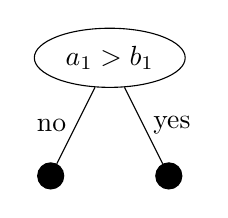
\begin{tikzpicture}
        \node[ellipse, draw] {$a_1 > b_1$}
            child {
                node[circle, draw, fill=black] {}
                edge from parent node[left] {no} 
            }
            child {
                node[circle, draw, fill=black] {}
                edge from parent node[right] {yes};
            };
    \end{tikzpicture}
    \caption{A node in a decision tree where we compare the elements $a_1$ and $b_1$ and proceed differently depending on which element is bigger.}
\end{figure}
In the decision tree, every node can be associated with a permutation of the list, each representing a different step in the sorting procedure (including those that do not sort the list). The leaf nodes represent a sorted list. 

If we are given an unsorted list of size $n$, then any of the $n!$ permutations of the list could be the sorted version of the list. Therefore, we need at least $n!$ distinct leaves, each leading to a different permutation of the unsorted list. We could have more leaves, but in that case there will be a permutation associated with more than one leaf.

This implies that the worst-case complexity of a sorting-based algorithm is $O(h)$, where $h$ is the height of the decision tree. An execution is a path from the root to the leaf node. Moreover, we need to perform an operation to go from one node to another, so we need to perform $h$ operations in the worst-case.

If we have a binary tree of height $h$, the it has at most $2^{h+1} - 1$ leaf nodes. We can prove this by induction:
\begin{itemize}
    \item If $h = 1$, then we have one node, which is a leaf. In that case, we have $n = 1 \leq 3 = 2^2 - 1 = 2^{h+1} - 1$.
    \item Now, assume that for some height $h$, every tree is of size $n_h \leq 2^{h+1} - 1$. Then, consider a tree of height $h+1$. It has at most $2n_h$ more nodes compared to a tree of height $h$. Therefore,
    \[n_{h+1} \leq 2\cdot n_h \leq 2 \cdot (2^{h+1} - 1) = 2^{h+2} - 2 \leq 2^{h+2} - 1.\]
    So, by induction, we find that a binary tree of height $h$ has at most $2^{h+1} - 1$ leaf nodes.
\end{itemize}

A decision tree is a binary tree (since every node has two branches- `yes' or `no'). Therefore, we find that
\[n! \leq 2^{h+1} - 1 \leq 2^{h+1}.\]
Taking $\log_2$ of both sides, we find that
\begin{align*}
    h+1 &\geq \log_2(n!) \\
    &\geq \log_2 (n/2)^{n/2} \\
    &= (n/2) \log_2 (n/2) \\
    &= (n/2) \log_2 n - (n/2) \log_2 2 \\
    &= (n/2) \log_2 n - n/2.
\end{align*}
This implies that $h$ is $O(n \log n)$. Here, we use the fact that $n! \geq \log_2 (n/2)^{n/2}$. We can see this as follows:
\begin{align*}
    n! &= n \cdot (n-1) \cdots (n/2) \cdot (n/2-1) \cdots  1 \\
    &\geq n \cdot (n-1) \cdots (n/2) \\
    &\geq (n/2) \cdot (n/2) \cdots (n/2) \\
    &= (n/2)^{n/2}.
\end{align*}

\subsection{Radix Sorting}
We have proven that no sorting algorithm based on comparison can be better than $O(n \log n)$ in the worst case. So, if we want to improve on this worst-case bound, we have to create a method based on something other than comparisons. 

Radix sorting uses a different approach to achieve $O(n)$ complexity. However, the algorithm has to exploit the structure of the items being sorted- it is less versatile. Moreover, in practice, it is faster than $O(n \log n)$ algorithms only for very large $n$.

This algorithm breaks down a number into smaller chunks with fewer digits, sorts them in place and continues sorting a more significant chunk. We consider sorting integers, but by transforming them into binary.

So, assume that every integer in the list can be written as a bit-sequence of length $m$. Moreover, let $b$ be a chosen factor of $m$. Here, $m$ and $b$ are constants for a particular instance. We can label each digit from $0$ to $m-1$, with bit $0$ being the most significant/leftmost bit. 

The algorithm iterates $m/b$ times. In each iteration, it places an element in one of the $2^b$ lists (or buckets), and joins each list to give the list to be used in the next iteration. The buckets correspond to a value between $0$ and $2^b - 1$. During the $i$-th iteration, the bits from position $b \cdot (i - 1)$ to $b \cdot i - 1$ are used to find the corresponding bucket. 

Since the buckets get concatenated starting from the bucket representing the smallest value and the sorting is in place, we end up with a sorted list after all the loop terminates.

Now, we apply the radix sorting algorithm to sort the list below.
\begin{figure}[H]
    \centering
    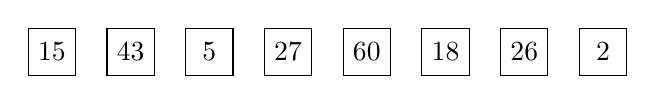
\begin{tikzpicture}
        \foreach \x[count=\i] in {15, 43, 5, 27, 60, 18, 26, 2} {
            \node at (\i, .5) {\x};
            \draw (\i-.3, .8) rectangle (\i+.3, .2);
        }
    \end{tikzpicture}
\end{figure}
\noindent First, we convert it into binary. The longest bit string is of length 6. So, we have $m = 6$. We choose $b = 2$. The list is shown below as bit strings.
\begin{figure}[H]
    \centering
    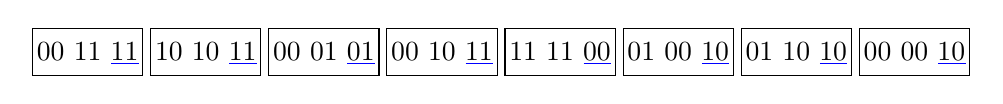
\begin{tikzpicture}
        \foreach \x[count=\i] in {00 11 11, 10 10 11, 00 01 01, 00 10 11, 11 11 00, 01 00 10, 01 10 10, 00 00 10} {
            \node at (\i*1.5, .5) {\x};
            \draw (1.5*\i-.7, .8) rectangle (1.5*\i+.7, .2);
            \draw[blue] (\i*1.5+.3, .35) -- (\i*1.5+.65, .35);
        }
    \end{tikzpicture}
\end{figure}
\noindent In this case, we have $2^2 = 4$ buckets: 00, 01, 10 and 11. In the first iteration, we add these numbers into the corresponding buckets based on positions $2 \cdot (1 - 1) = 0$ to $2 \cdot 1 - 1 = 1$.
\begin{table}[H]
    \centering
    \begin{tabular}{c|rrr}
        00 & 60=1111{\color{red}00} \\
        \hline
        01 & 5=0001{\color{red}01} \\
        \hline
        10 & 18=0100{\color{red}10} & 26=0110{\color{red}10} & 2=0000{\color{red}10} \\
        \hline
        11 & 15=0011{\color{red}11} & 43=1010{\color{red}11} & 27=0010{\color{red}11}
    \end{tabular}
\end{table}
\noindent We now concatenate the buckets to get the list we will use in the next iteration.
\begin{figure}[H]
    \centering
    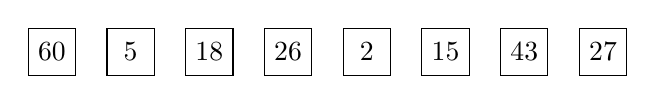
\begin{tikzpicture}
        \foreach \x[count=\i] in {60, 5, 18, 26, 2, 15, 43, 27} {
            \node at (\i, .5) {\x};
            \draw (\i-.3, .8) rectangle (\i+.3, .2);
        }
    \end{tikzpicture}
\end{figure}
\noindent The binary representation of the list is now the following.
\begin{figure}[H]
    \centering
    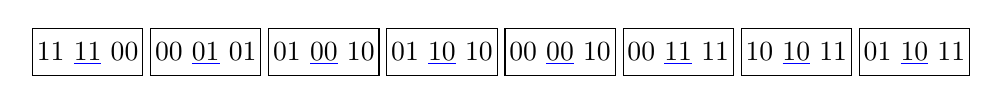
\begin{tikzpicture}
        \foreach \x[count=\i] in {11 11 00, 00 01 01, 01 00 10, 01 10 10, 00 00 10, 00 11 11, 10 10 11, 01 10 11} {
            \node at (\i*1.5, .5) {\x};
            \draw (1.5*\i-.7, .8) rectangle (1.5*\i+.7, .2);
            \draw[blue] (\i*1.5-.175, .35) -- (\i*1.5+.175, .35);
        }
    \end{tikzpicture}
\end{figure}
\noindent We are now in the second iteration. So, we are considering the positions $2 \cdot (2 - 1) = 2$ to $2 \cdot 2 - 1 = 3$, as highlighted in blue above. We place them in the four buckets depending on the value within the highlighted position, and that gives us the following list of buckets.
\begin{table}[H]
    \centering
    \begin{tabular}{c|rrr}
        00 & 18=01{\color{red}00}10 & 2=00 {\color{red}00} 10  \\
        \hline
        01 & 5=00{\color{red}01}01 \\
        \hline
        10 & 26=01{\color{red}10}10 & 43=10{\color{red}10}11 & 27=01{\color{red}10}11 \\
        \hline
        11 & 60=11{\color{red}11}00 & 15=00{\color{red}11}11
    \end{tabular}
\end{table}
\noindent Note that the value $26$ comes before $27$ since $26$ came before $27$ in the list at the start of this iteration. This happens because we are sorting in place. Concatenating this, we get the following list.
\begin{figure}[H]
    \centering
    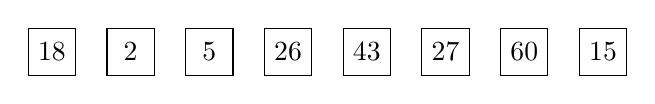
\begin{tikzpicture}
        \foreach \x[count=\i] in {18, 2, 5, 26, 43, 27, 60, 15} {
            \node at (\i, .5) {\x};
            \draw (\i-.3, .8) rectangle (\i+.3, .2);
        }
    \end{tikzpicture}
\end{figure}
\noindent The list in binary, with the highlighted positions $4$ and $5$, is shown below.
\begin{figure}[H]
    \centering
    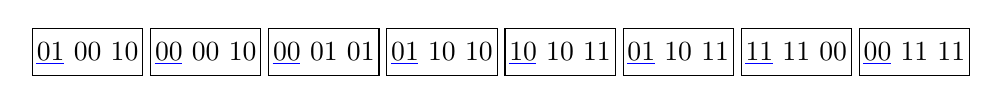
\begin{tikzpicture}
        \foreach \x[count=\i] in {01 00 10, 00 00 10, 00 01 01, 01 10 10, 10 10 11, 01 10 11, 11 11 00, 00 11 11} {
            \node at (\i*1.5, .5) {\x};
            \draw (1.5*\i-.7, .8) rectangle (1.5*\i+.7, .2);
            \draw[blue] (\i*1.5-.65, .35) -- (\i*1.5-.3, .35);
        }
    \end{tikzpicture}
\end{figure}
\noindent Now, we are in the final iteration. In total, there were $m/b = 6/2 = 3$ iterations. We add each element in the list into the bucket.
\begin{table}[H]
    \centering
    \begin{tabular}{c|rrr}
        00 & 2={\color{red}00}0010 & 5={\color{red}00}0101 \\
        \hline
        01 & 18={\color{red}01}0010 & 26={\color{red}01}1010 & 27= {\color{red}01} 1011 \\
        \hline
        10 & 43={\color{red}10}1011 \\
        \hline
        11 & 60={\color{red}11}1100
    \end{tabular}
\end{table}
\noindent We then concatenate the list.
\begin{figure}[H]
    \centering
    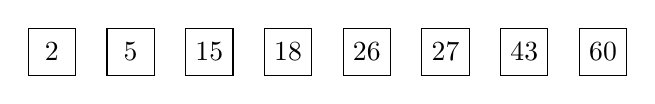
\begin{tikzpicture}
        \foreach \x[count=\i] in {2, 5, 15, 18, 26, 27, 43, 60} {
            \node at (\i, .5) {\x};
            \draw (\i-.3, .8) rectangle (\i+.3, .2);
        }
    \end{tikzpicture}
\end{figure}
\noindent This gives us the sorted list.

The pseudocode for radix sorting is given below.
\lstinputlisting[language=pseudocode]{src/radixSort.psc}

Next, we show that radix sorting is correct. That is, if we have $x$ and $y$ in a list with $x < y$, then we need to show that $x$ precedes $y$ in the final sequence. Suppose that $j$ is the last iteration for which $x$ and $y$ differ (i.e. every bit after $j$ is the same in $x$ and $y$). Since $x < y$, the relevant bits of $x$ must be smaller than those of $y$. Therefore, $x$ goes to an `earlier' bucket that $y$- after concatenation, $x$ precedes $y$ in the sequence after this iteration. Since any bit after this is the same in both $x$ and $y$, they will both end up at the same bucket. Since the algorithm is in-place, $x$ will still precede $y$ at the end. Therefore, the final list will be sorted.

Finally, we consider the complexity of radix sort. The number of iterations is $m/b$ and the number of buckets is $2^b$. In each iteration, we scan the sequence and add them to one of the buckets- this takes $O(n)$ time. The buckets then get concatenated- this takes $O(2^b)$ time. So, the overall complexity is $O(m/b \cdot (n + 2^b))$. Since $m$ and $b$ are constants, this simplifies to $O(n)$.

When choosing the value $b$, there is a time-space trade-off. If we choose a large value of $b$, the multiplicative constant $m/b$ will be small. So, the algorithm will become faster. But, we will need an array of size $2^b$- this increases the space requirements exponentially.
\newpage

\section{Tries}
A trie is used to store items that can be interpreted as a sequence of bits or characters. There is a multi-way branch at each node where each branch has an associated symbol and no two siblings have the same symbol. The branch taken at level $i$ during a search is determined by the $i$-th element of the value ($i$-th bit, $i$-th character, etc.). Tracing a path from the root to a node spells out the value of the item. 

A trie can be used to store items with string values, e.g. words in a dictionary. An example is of a trie is given below.
\begin{figure}[H]
    \centering
    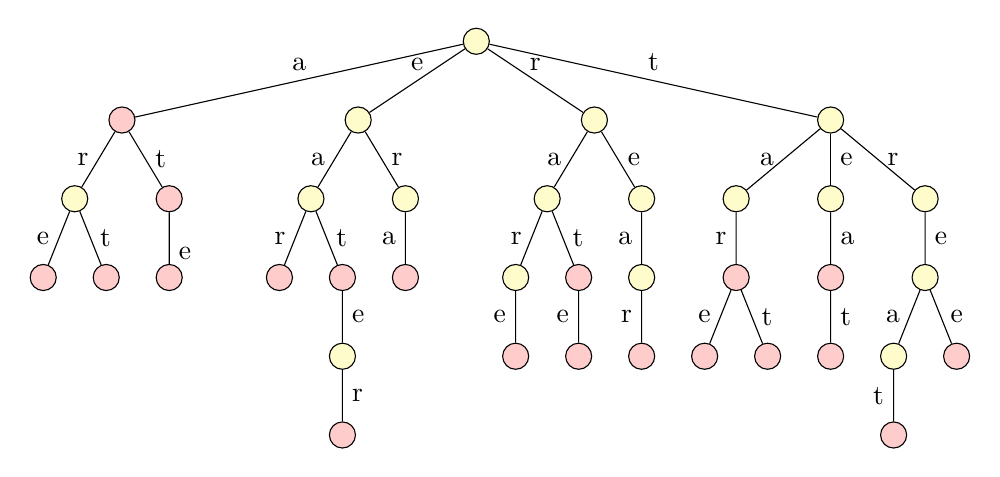
\begin{tikzpicture}[
        level 1/.style = {sibling distance = 3cm},
        level 2/.style = {sibling distance = 1.2cm},
        level 3/.style = {sibling distance = .8cm},
    ]
        \node[circle, draw, fill=yellow!20] {} [level distance=1cm]
            child {
                node[circle, draw, fill=red!20] {}
                child {
                    node[circle, draw, fill=yellow!20] {}
                    child {
                        node[circle, draw, fill=red!20] {}
                        edge from parent node[left] {e}
                    }
                    child {
                        node[circle, draw, fill=red!20] {}
                        edge from parent node[right] {t}
                    }
                    edge from parent node[left] {r}
                }
                child {
                    node[circle, draw, fill=red!20] {}
                    child {
                        node[circle, draw, fill=red!20] {}
                        edge from parent node[below right] {e}
                    }
                    edge from parent node[right] {t}
                }
                edge from parent node[above] {a}
            }
            child {
                node[circle, draw, fill=yellow!20] {}
                child {
                    node[circle, draw, fill=yellow!20] {}
                    child {
                        node[circle, draw, fill=red!20] {}
                        edge from parent node[left] {r}
                    }
                    child {
                        node[circle, draw, fill=red!20] {}
                        child {
                            node[circle, draw, fill=yellow!20] {}
                            child {
                                node[circle, draw, fill=red!20] {}
                                edge from parent node[right] {r}
                            }
                            edge from parent node[right] {e}
                        }
                        edge from parent node[right] {t}
                    }
                    edge from parent node[left] {a}
                }
                child {
                    node[circle, draw, fill=yellow!20] {}
                    child {
                        node[circle, draw, fill=red!20] {}
                        edge from parent node[left] {a}
                    }
                    edge from parent node[right] {r}
                }
                edge from parent node[above] {e}
            }
            child {
                node[circle, draw, fill=yellow!20] {}
                child {
                    node[circle, draw, fill=yellow!20] {}
                    child {
                        node[circle, draw, fill=yellow!20] {}
                        child {
                            node[circle, draw, fill=red!20] {}
                            edge from parent node[left] {e}
                        }
                        edge from parent node[left] {r}
                    }
                    child {
                        node[circle, draw, fill=red!20] {}
                        child {
                            node[circle, draw, fill=red!20] {}
                            edge from parent node[left] {e}
                        }
                        edge from parent node[right] {t}
                    }
                    edge from parent node[left] {a}
                }
                child {
                    node[circle, draw, fill=yellow!20] {}
                    child {
                        node[circle, draw, fill=yellow!20] {}
                        child {
                            node[circle, draw, fill=red!20] {}
                            edge from parent node[left] {r}
                        }
                        edge from parent node[left] {a}
                    }
                    edge from parent node[right] {e}
                }
                edge from parent node[above] {r}
            }
            child {
                node[circle, draw, fill=yellow!20] {}
                child {
                    node[circle, draw, fill=yellow!20] {}
                    child {
                        node[circle, draw, fill=red!20] {}
                        child {
                            node[circle, draw, fill=red!20] {}
                            edge from parent node[left] {e}
                        }
                        child {
                            node[circle, draw, fill=red!20] {}
                            edge from parent node[right] {t}
                        }
                        edge from parent node[left] {r}
                    }
                    edge from parent node[left] {a}
                }
                child {
                    node[circle, draw, fill=yellow!20] {}
                    child {
                        node[circle, draw, fill=red!20] {}
                        child {
                            node[circle, draw, fill=red!20] {}
                            edge from parent node[right] {t}
                        }
                        edge from parent node[right] {a}
                    }
                    edge from parent node[right] {e}
                }
                child {
                    node[circle, draw, fill=yellow!20] {}
                    child {
                        node[circle, draw, fill=yellow!20] {}
                        child {
                            node[circle, draw, fill=yellow!20] {}
                            child {
                                node[circle, draw, fill=red!20] {}
                                edge from parent node[left] {t}
                            }
                            edge from parent node[left] {a}
                        }
                        child {
                            node[circle, draw, fill=red!20] {}
                            edge from parent node[right] {e}
                        }
                        edge from parent node[right] {e}
                    }
                    edge from parent node[right] {r}
                }
                edge from parent node[above] {t}
            };
    \end{tikzpicture}
    \caption{A Trie}
\end{figure}
We follow a path to spell out a word from left to right. A red node represents values that are words, while a yellow node represents an intermediate node. So, \texttt{tree} is a word but \texttt{trea} is not.

The search algorithm in a trie is given below:
\lstinputlisting[language=pseudocode]{src/trieSearch.psc}
The insertion algorithm in a trie is given below:
\lstinputlisting[language=pseudocode]{src/trieInsert.psc}
The deletion algorithm in a trie is given below:
\lstinputlisting[language=pseudocode]{src/trieDelete.psc}
Most trie operations are independent of the number of items present. They are essentially linear in the length of the string.
There are various possible implementations of a trie, e.g. arrays or linked lists. In a linked list implementation, a node stores the character it represents, along with pointers to the next child of the parent node (called its sibling) and the (first) child of this node. The code can be optimised by sorting the children nodes using the lexicographic order of the character.

\end{document}
